% AJ manuscript -- AASTeX. Compile with: latexmk -pdf ms.tex  (needs aastex701.cls)
% Draft generated 2026-06-16. Numbers from the frozen DES test split unless noted.
\documentclass[twocolumn]{aastex701}

\shorttitle{An Amortized Continuous PSF Field for DES}
\shortauthors{Regier et al.}

\usepackage{tikz}
\usetikzlibrary{positioning,arrows.meta,fit,backgrounds,calc}

\begin{document}

\title{An Amortized Continuous PSF Field for DES Single-Epoch Imaging}

\author{Jeffrey Regier}
\email{regier@umich.edu}
\affiliation{Department of Statistics, University of Michigan, Ann Arbor, MI 48109, USA}

\author{[Collaborators]}
\email{collaborator@example.edu}
\affiliation{[Affiliation]}

\begin{abstract}
Accurate point-spread-function (PSF) models are the dominant systematic in weak-lensing
shear measurement. The standard approach fits an independent PSF model per exposure
(e.g., \textsc{PSFEx}, \textsc{PIFF}) from that exposure's stars. We instead learn a
single \emph{amortized} continuous PSF field: a multi-head attention network takes an
exposure's stars as context (position, color, flux, and pixel cutouts) and predicts the
PSF at any queried position and resolution, with no per-exposure fitting at test time.
On 3{,}301 frozen test exposures of Dark Energy Survey (DES) single-epoch imaging
(CCD~31, $grizY$; 73{,}609 reserved stars), the model matches or exceeds \textsc{PIFF}
and \textsc{PSFEx} on every metric: size-residual scatter $0.030$ versus $0.039/0.037$,
ellipticity errors $|\delta e_1|,|\delta e_2|=0.015/0.015$ versus $0.017/0.016$
(\textsc{PIFF}), and shape correlations $0.65/0.61$ versus $0.61/0.58$ (\textsc{PIFF}),
at $\chi^2/{\rm dof}=1.04$. In a star-anchored galaxy injection--recovery test on real
data, our PSF recovers galaxy \emph{ellipticity} far better than \textsc{PIFF}
($\Delta e_1=+0.004$ versus $-0.138$), the weak-lensing-critical quantity. Color
conditioning removes a chromatic PSF-size systematic that the baselines retain
($+0.004$/mag versus $\sim\!-0.06$/mag residual slope). The model is flat in the number
of available fit stars where \textsc{PIFF} degrades sharply ($\chi^2\simeq1.1$ versus
$5.1$ at five stars). Using simulations as a controlled instrument, we show that a
\emph{blend forward-model} training loss removes a size bias from unrecognized blends,
and we identify and fix a spin-2 representation failure in which the network corrupts the
PSF ellipticity by attending to galaxy detections in its context; restricting attention
to point sources recovers it fully.
\end{abstract}

\keywords{Weak gravitational lensing (1797) --- Point spread function (1349) ---
Astronomical techniques (1684) --- Convolutional neural networks (1938) ---
Sky surveys (1464)}

\section{Introduction} \label{sec:intro}

Weak gravitational lensing infers the matter distribution from coherent ${\sim}1\%$
distortions of galaxy shapes. The measurement is limited by knowledge of the PSF: any
error in the modeled PSF size or ellipticity propagates directly into the inferred shear.
Survey pipelines model the PSF per exposure by fitting that exposure's stars with a
flexible model interpolated across the focal plane \citep[\textsc{PSFEx};][]{Bertin2011}
\citep[\textsc{PIFF};][]{Jarvis2021}. This is robust but (i)~discards information shared
across exposures and nights, (ii)~degrades when few clean stars are available, and
(iii)~is purely empirical at the star positions---it does not exploit auxiliary
information such as stellar color, which sets the chromatic PSF.

We take an amortized, learning-based approach. A single network is trained across many
exposures to map an exposure's stars (the \emph{context}) to a continuous PSF field,
queryable at arbitrary position, color, flux, and resolution. The inferential target is
the PSF at \emph{star-free} positions, where galaxies are measured; predicting held-out
stars is the training objective and the validation instrument. We train and evaluate on
DES single-epoch data and benchmark against \textsc{PIFF} and \textsc{PSFEx} run by us
under matched conditions.
\begin{figure*}
\centering
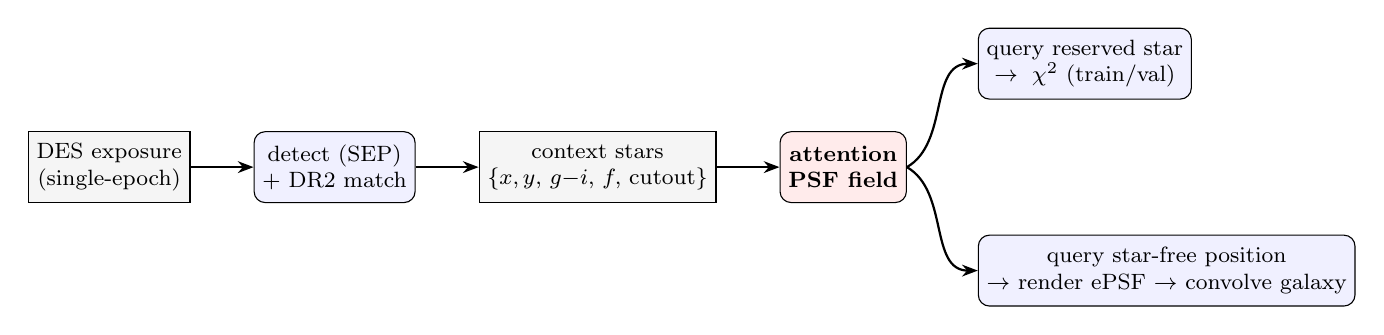
\begin{tikzpicture}[
  node distance=5mm and 8mm,
  box/.style={draw, rounded corners, align=center, minimum height=9mm,
              font=\footnotesize, fill=blue!6, inner sep=3pt},
  dat/.style={draw, align=center, minimum height=9mm, font=\footnotesize,
              fill=gray!8, inner sep=3pt},
  net/.style={draw, rounded corners, align=center, minimum height=9mm,
              font=\footnotesize\bfseries, fill=red!8, inner sep=3pt},
  arr/.style={-{Stealth[length=2mm]}, thick}]
\node[dat] (exp) {DES exposure\\(single-epoch)};
\node[box, right=of exp] (det) {detect (SEP)\\+ DR2 match};
\node[dat, right=of det] (ctx) {context stars\\$\{x,y,\,g{-}i,\,f,\,\mathrm{cutout}\}$};
\node[net, right=of ctx] (npsf) {attention\\PSF field};
\node[box, above right=4mm and 9mm of npsf] (res)
  {query reserved star\\$\to\ \chi^2$ \footnotesize(train/val)};
\node[box, below right=4mm and 9mm of npsf] (gal)
  {query star-free position\\$\to$ render ePSF $\to$ convolve galaxy};
\draw[arr] (exp)--(det); \draw[arr] (det)--(ctx); \draw[arr] (ctx)--(npsf);
\draw[arr] (npsf.east) to[out=30,in=180] (res.west);
\draw[arr] (npsf.east) to[out=-30,in=180] (gal.west);
\end{tikzpicture}
\caption{Overall workflow. A single network, trained across exposures, maps an
exposure's detected stars (context) to a continuous PSF field. Querying held-out reserved
stars provides the training objective and validation; the inferential target is the PSF
at star-free positions, rendered (oversampled) to convolve galaxy models.\label{fig:workflow}}
\end{figure*}



\section{Method} \label{sec:method}
\begin{figure*}
\centering
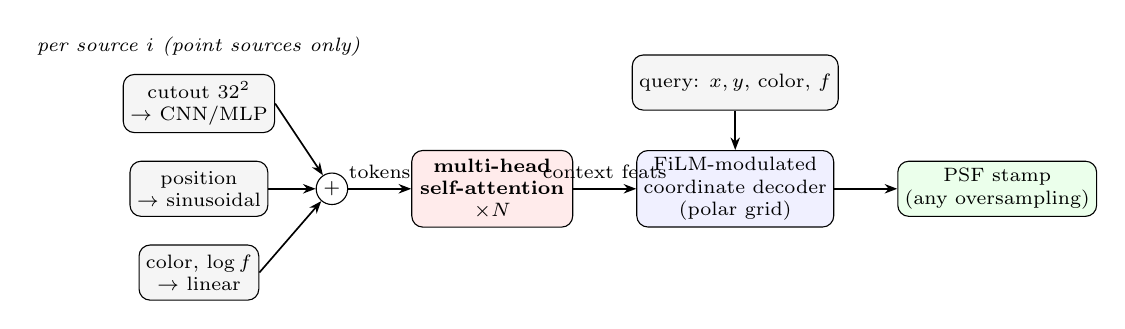
\begin{tikzpicture}[
  node distance=3.5mm and 7mm,
  enc/.style={draw, rounded corners, align=center, minimum height=7mm,
              font=\scriptsize, fill=gray!8, inner sep=2.5pt},
  op/.style={draw, circle, font=\scriptsize, inner sep=1pt, minimum size=4mm, fill=white},
  att/.style={draw, rounded corners, align=center, minimum height=9mm,
              font=\scriptsize\bfseries, fill=red!8, inner sep=3pt},
  dec/.style={draw, rounded corners, align=center, minimum height=7mm,
              font=\scriptsize, fill=blue!6, inner sep=2.5pt},
  arr/.style={-{Stealth[length=1.6mm]}, semithick}]
% per-source token encoder
\node[enc] (cut) {cutout $32^2$\\$\to$ CNN/MLP};
\node[enc, below=of cut] (pos) {position\\$\to$ sinusoidal};
\node[enc, below=of pos] (sca) {color, $\log f$\\$\to$ linear};
\node[op, right=6mm of pos] (sum) {$+$};
\draw[arr] (cut.east) -- (sum); \draw[arr] (pos.east) -- (sum); \draw[arr] (sca.east) -- (sum);
\node[align=center, font=\scriptsize, above=1mm of cut] {\emph{per source $i$ (point sources only)}};
\node[att, right=8mm of sum] (mha) {multi-head\\self-attention\\$\times N$};
\draw[arr] (sum) -- node[above, font=\scriptsize]{tokens} (mha);
\node[dec, right=8mm of mha] (film) {FiLM-modulated\\coordinate decoder\\(polar grid)};
\draw[arr] (mha) -- node[above, font=\scriptsize]{context feats} (film);
\node[enc, above=5mm of film] (q) {query: $x,y$, color, $f$};
\draw[arr] (q) -- (film);
\node[dec, right=8mm of film, fill=green!8] (psf) {PSF stamp\\(any oversampling)};
\draw[arr] (film) -- (psf);
\end{tikzpicture}
\caption{Network architecture. Each context source (restricted to point sources;
\S\ref{sec:method}) is encoded from its pixel cutout, sky position, and scalar
color/$\log$-flux into a token. Multi-head self-attention mixes the context; a
FiLM-modulated coordinate decoder, conditioned on the attended features and the query
(position, color, flux), renders the pixel-convolved PSF at any position and oversampling
factor.\label{fig:arch}}
\end{figure*}



\paragraph{Architecture} Each detected source is encoded from its pixel cutout (a learned
image encoder applied to the scale-normalized stamp), its sky position (sinusoidal
encoding), and scalar color and $\log$-flux. A multi-head self-attention block lets every
query attend to the context sources; a coordinate decoder then renders the PSF at the
query position and any oversampling factor, returning the pixel-convolved effective PSF
used to convolve galaxy models. We use a polar (spin-2-aware) angular parametrization of
the decoder and FiLM modulation of the decoder by the attended context features.

\paragraph{Loss} Training minimizes an inverse-variance $\chi^2$ between predicted and
observed star cutouts, with the per-star amplitude solved in closed form. We introduce a
\emph{blend forward-model} loss: rather than treat each clean star as isolated, we model
its cutout as a generalized-least-squares sum of the target plus its detected neighbors,
all rendered by the same decoder (\S\ref{sec:sim}). Detected galaxies near a target are
handled by exclusion (default), masking, or a crude extended-component model; the three
are within noise on real reserved stars.

\paragraph{Point-source context} The PSF should be informed only by point sources. We
restrict the attention context to stellar detections; \S\ref{sec:sim} shows this is
necessary to avoid a spin-2 corruption from extended sources in the context.

\paragraph{Color conditioning} The decoder conditions on $g{-}i$ color, enabling a
per-object chromatic PSF (differential chromatic refraction and wavelength-dependent
seeing) that per-exposure empirical models cannot represent (\S\ref{sec:chromatic}).

\section{Data} \label{sec:data}

We use DES single-epoch FITS (Y5A1, CCD~31; amplifier~B is dead, masked via MSK bit~8).
Sources are detected with \textsc{SEP} and cross-matched to DES~DR2 for colors,
\texttt{SPREAD\_MODEL} star/galaxy labels, and coadd object IDs. Splits are at the
observing-night level by deterministic hash to prevent leakage (consecutive exposures
share atmosphere), frozen in a committed manifest with ${\sim}20\%$ of clean stars per
test/validation exposure reserved for scoring only; the test split is 3{,}301 exposures
across $grizY$. Reserved stars are excluded from every method's fit/context and scored
identically across methods on the same pixel grid.

\paragraph{Simulations} A matched pipeline renders Moffat PSF fields (second-order
polynomial FWHM and shear variation---exactly representable by \textsc{PIFF}/\textsc{PSFEx},
a deliberately fair-to-baselines choice) into the same data format, optionally with
chromatic FWHM--color dependence, blended stars, and injected galaxy detections. Star
density, galaxy density ($3{:}1$), and per-source S/N are tuned to match the real
extraction. The simulation is the controlled instrument for the systematics studies in
\S\ref{sec:sim}.


\begin{figure*}
\centering
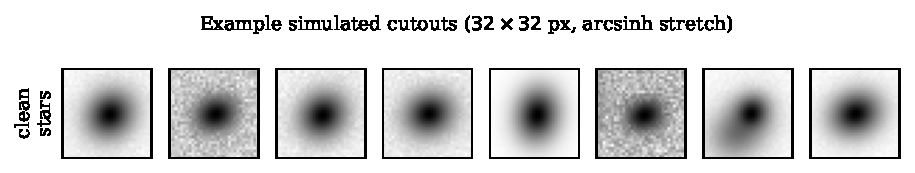
\includegraphics[width=\textwidth]{figures/fig_simdata.pdf}
\caption{Example simulated cutouts. Clean stars (top) are compact point sources; injected galaxies (bottom) are visibly extended and elliptical (second-moment size $T\approx33$ vs $15\,$px$^2$). Both are presented to the network as context.\label{fig:simdata}}
\end{figure*}


\begin{figure}
\centering

\includegraphics[width=\columnwidth]{figures/fig_psffield.pdf}
\caption{The true, spatially varying PSF ellipticity field in a simulated exposure (whisker length $\propto|e|$); the network must recover this at star-free positions.\label{fig:psffield}}
\end{figure}

\section{Results} \label{sec:results}

\subsection{Reserved-star accuracy on real data} \label{sec:headline}

On 3{,}301 test exposures and 73{,}609 reserved stars, the amortized model (no
per-exposure fitting) matches or exceeds both baselines on every metric
(Table~\ref{tab:headline}). Reserved ``clean'' stars carry a mild blend-contamination
floor that suppresses absolute correlations for \emph{all} methods; the comparison is
fair (identical stars) and the ordering is robust.
\begin{figure*}
\centering
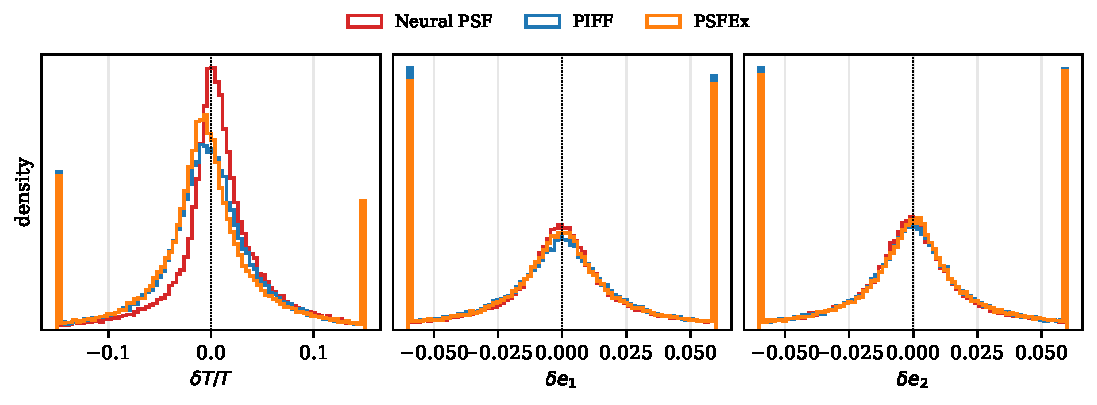
\includegraphics[width=\textwidth]{figures/fig_residuals.pdf}
\caption{Reserved-star residual distributions on the DES test split. Our amortized model (red) is the narrowest in size and ellipticity.\label{fig:residuals}}
\end{figure*}



\begin{deluxetable}{lcccccc}
\tablecaption{Reserved-star residuals on the DES test split (3{,}301 exposures,
73{,}609 stars). $T$ scatter is the robust standard deviation of $\delta T/T$;
$|\delta e|$ are median absolute ellipticity residuals; corr is the model--star shape
correlation. Best in bold.\label{tab:headline}}
\tablehead{\colhead{Method} & \colhead{$T$ scat} & \colhead{$|\delta e_1|$} &
\colhead{$|\delta e_2|$} & \colhead{corr$(e_1)$} & \colhead{corr$(e_2)$} &
\colhead{$\chi^2/$dof}}
\startdata
\textbf{This work} & \textbf{0.0301} & \textbf{0.0151} & \textbf{0.0150} &
  \textbf{0.650} & \textbf{0.607} & 1.037 \\
\textsc{PIFF}      & 0.0393 & 0.0171 & 0.0158 & 0.611 & 0.577 & 1.073 \\
\textsc{PSFEx}     & 0.0371 & 0.0160 & 0.0154 & 0.645 & 0.604 & 1.047 \\
\enddata
\end{deluxetable}

\subsection{Galaxy recovery on real data} \label{sec:galrec}

We test the inferential goal directly. We inject \textsc{galsim} galaxies, convolved with
a strictly isolated reserved star's empirical PSF, at that star's position; each method
predicts the PSF there from the \emph{other} stars and recovers the galaxy. The truth arm
(the anchor's own image) recovers near-zero bias, validating the protocol. On 113 $r$-band
exposures and 522 anchors (Table~\ref{tab:galrec}), our PSF recovers galaxy
\emph{ellipticity} essentially without bias, whereas \textsc{PIFF}'s PSF-ellipticity error
induces a large shape bias ($\Delta e_1=-0.14$). \textsc{PIFF} recovers size slightly
better; our PSF is ${\sim}6\%$ too broad at star-free positions. For weak lensing, the
ellipticity result is the consequential one.
\begin{figure}
\centering

\includegraphics[width=\columnwidth]{figures/fig_galrec.pdf}
\caption{Galaxy ellipticity recovery on real data (star-anchored injection). PIFF's PSF-ellipticity error biases recovered galaxy $e_1$ by $-0.14$; ours is unbiased.\label{fig:galrec}}
\end{figure}



\begin{deluxetable}{lccc}
\tablecaption{Star-anchored galaxy injection--recovery (113 $r$-band exposures, 522
anchors). The truth arm validates the protocol.\label{tab:galrec}}
\tablehead{\colhead{Arm} & \colhead{Size bias} & \colhead{$\Delta e_1$} &
\colhead{$\Delta e_2$}}
\startdata
Truth (validation) & $-1.5\%$ & $-0.002$ & ${\sim}0$ \\
\textbf{This work}  & $-7.6\%$ & $\mathbf{+0.004}$ & $-0.002$ \\
\textsc{PIFF}       & $-1.0\%$ & $\mathbf{-0.138}$ & $-0.001$ \\
\enddata
\end{deluxetable}

\subsection{Chromatic PSF correction} \label{sec:chromatic}

In a chromatic simulation (FWHM varies $-3\%$/mag of $g{-}i$), color conditioning reduces
the residual chromatic size slope from $-0.06$/mag (\textsc{PIFF}, \textsc{PSFEx}, and our
own zero-color ablation) to $+0.004$/mag---a ${\sim}17\times$ reduction. On real $r$-band
data the paired color-versus-zero-color slope difference is $+0.0024$/mag
(CI $[+0.0016,+0.0030]$); the baselines structurally retain the systematic. This is
information unavailable to a per-exposure empirical PSF.

\subsection{Sample efficiency} \label{sec:sampeff}

Restricting every method to $k$ randomly chosen fit stars, the amortized model is
approximately flat in $k$ (size scatter $0.078\to0.056$, $\chi^2\sim1.1$ from $k=5$ to
$k=100$), while \textsc{PIFF} collapses below $k\approx25$ ($\chi^2=5.1$, scatter $0.18$
at $k=5$). Amortization transfers information from the training set to sparsely-populated
exposures.


\begin{figure}
\centering

\includegraphics[width=\columnwidth]{figures/fig_sampeff.pdf}
\caption{Size-residual scatter versus the number of fit stars $k$. The amortized model is nearly flat in $k$; PIFF degrades sharply below $k\approx25$.\label{fig:sampeff}}
\end{figure}

\subsection{Simulation studies} \label{sec:sim}

\paragraph{Architecture ladder} On the star-free truth grid, $\chi^2/$dof improves along
additive $\to$ FiLM $\to$ diagonal $\to$ polar ($8.9\to4.96\to4.41$; \textsc{PIFF} $2.67$;
verified floor $1.0$), recovering both ellipticity components.

\paragraph{Blend forward-model} On a blended simulation, single-star training leaves a
$+4.8\%$ size bias on the star-free truth grid; the blend forward-model loss reduces it to
$+0.7\%$ (${\approx}7\times$).

\paragraph{Galaxy-context corrupts PSF ellipticity---and the fix} Injecting galaxy
detections into the simulation, a model that attends to \emph{all} detections (including
galaxies) suffers a clean, reproducible failure: it cannot represent one spin-2
ellipticity component [corr$(e_1)=0.05$ under the polar parametrization; the failure flips
to $e_2$ under a Cartesian parametrization, identifying a representation degeneracy rather
than noise], while recovering the other perfectly. We localize the cause by ablation: it
is \emph{not} data volume, per-source S/N, galaxy size or color, or the $\chi^2$ cap---the
model is treating extended galaxy cutouts as PSF evidence. Restricting the attention
context to point sources recovers \emph{both} components completely
[corr$(e_1,e_2)=0.98$, matching the galaxy-free ideal]; a coordinate-system change does
not. Galaxies are clearly distinguishable (cutout second moment $T\approx33$ versus
$15\,{\rm px}^2$ for stars), so this is the model failing to use available information,
fixed by the principled restriction that only point sources inform a PSF.
\begin{figure*}
\centering
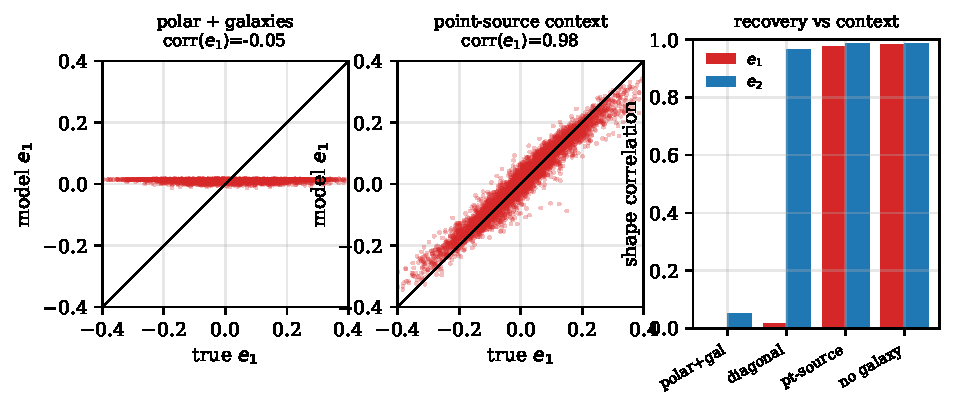
\includegraphics[width=\textwidth]{figures/fig_galaxy_context.pdf}
\caption{Galaxy detections in the attention context corrupt the recovered PSF ellipticity. Left: with galaxies in context, model $e_1$ collapses to a constant (corr$=-0.04$). Middle: restricting the context to point sources recovers it (corr$=0.98$). Right: shape correlations across configurations---point-source context and galaxy-free both recover \emph{both} components; a coordinate change (diagonal) does not.\label{fig:galcontext}}
\end{figure*}



\section{Discussion} \label{sec:discussion}

The amortized field trades a per-exposure fit for a single trained model. Benefits: no
test-time fitting, robustness in star-sparse exposures, and conditioning on color
(chromatic PSF) and flux (brighter--fatter). Caveats: (i)~unlike per-exposure fitters, the
amortized model requires many exposures to learn the field (in simulation, ellipticity
recovery is unstable below a few thousand exposures; real DES is well above this);
(ii)~the simulation's idealized PSF (Moffat, low-order polynomial field) favors the
per-exposure baselines, so absolute-accuracy comparisons rest on real data; and
(iii)~the galaxy-context finding argues that a PSF estimator's context should be gated to
point sources, which we adopt.

\section{Conclusion} \label{sec:conclusion}

A single attention-based continuous PSF field, trained across DES single-epoch exposures
and applied with no per-exposure fitting, matches or exceeds \textsc{PIFF} and
\textsc{PSFEx} on real reserved stars and recovers galaxy ellipticity better than
\textsc{PIFF} on a star-anchored injection test, while additionally correcting a chromatic
systematic and remaining robust in star-sparse exposures. Controlled simulations motivate
two training choices---a blend forward-model loss and point-source-only attention
context---the latter from a clean diagnosis of a spin-2 representation failure triggered
by galaxy detections in context.

\begin{acknowledgments}
[Acknowledgments, funding, DES consortium statement.] Baselines: \textsc{PIFF} (PixelGrid,
second-order \texttt{BasisPolynomial}, $4\sigma$ rejection) and \textsc{PSFEx}
(\texttt{PSF\_SAMPLING}~0.5, $45\times45$, \texttt{PSFVAR\_DEGREES}~2; rendered via
\textsc{galsim} \texttt{DES\_PSFEx}, \texttt{method='no\_pixel'}).
\end{acknowledgments}

\software{Astropy \citep{Astropy2022}, GalSim \citep{Rowe2015}, SEP \citep{Barbary2016},
PyTorch \citep{Paszke2019}, PIFF \citep{Jarvis2021}, PSFEx \citep{Bertin2011}}

\bibliographystyle{aasjournalv7}
\bibliography{ms}

\end{document}
